% \section{Investigating Task Computation Requirements}

% \label{sec:taskcompresults}
% % \subsection{Main Results: Relationship Between \cname and Method Complexity}

% Now that we've set things up, and shown what results look like for an example $O(N^2)$ \cname task, we can now address our central question: \textbf{how do tasks with different \cname requirements interact with different complexity of computation}? To keep things simple, we'll look at just standard vs chunked attention, at model scales where both are sufficiently capable of tasks. If our hypothesis is true, then we'll expect $O(N)$ tasks to show little degradation over scale, even with chunked attention, and any gap should remain similar across scale. For $O(NM)$ tasks we may expect the gap to widen as both N and M increase (if M doesn't increase then it should behave like an $O(N)$ task). And for $O(N^2)$ tasks the gap should widen more dramatically at high enough contexts.

% \begin{figure}[t]
% \centering
% 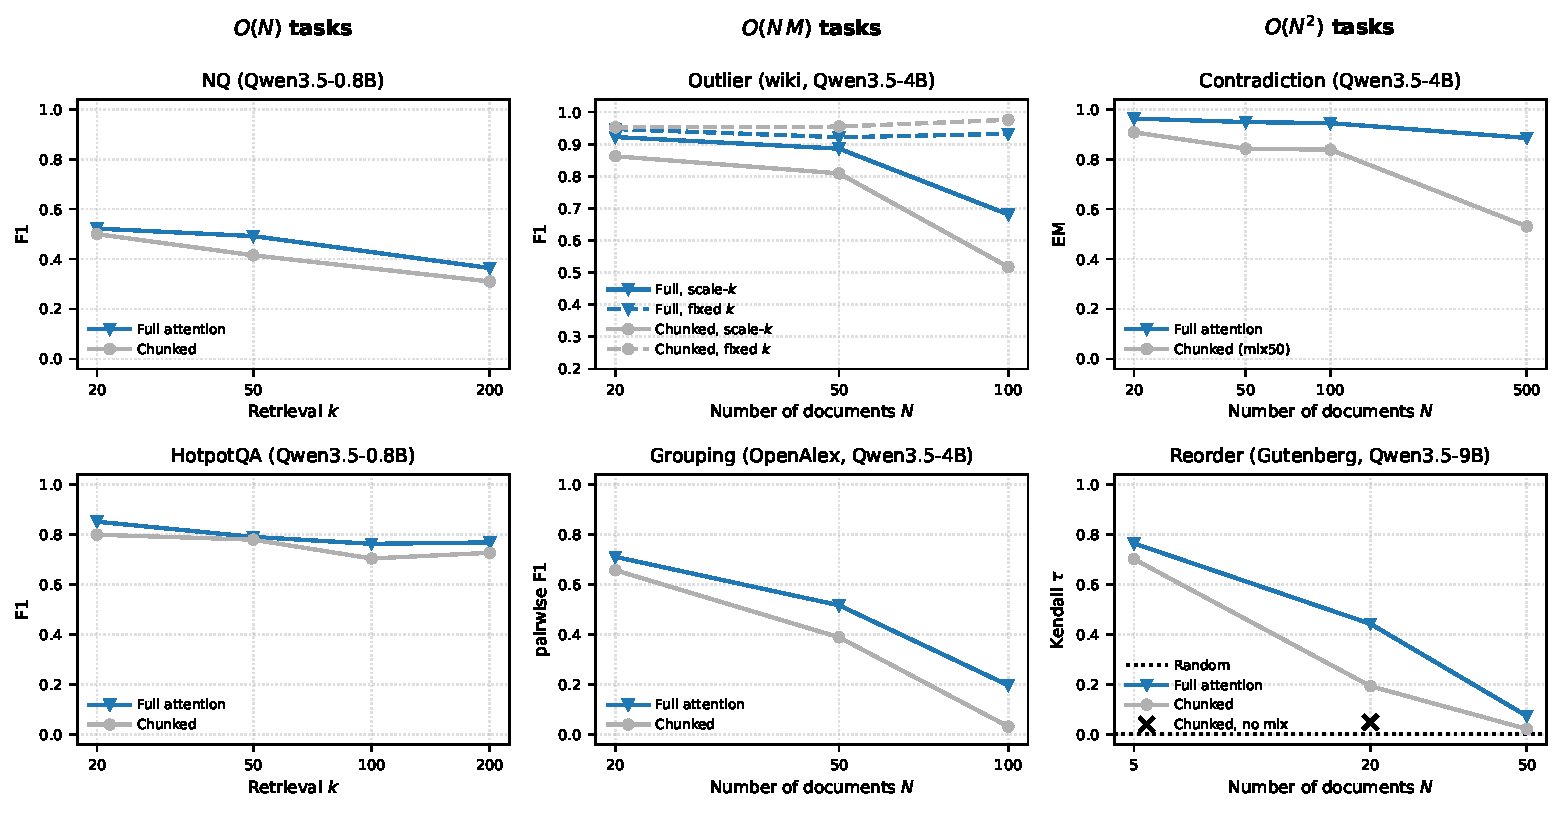
\includegraphics[width=\textwidth]{figures/section5_cross_task.pdf}
% \caption{\textbf{Cross-task scaling of full vs.\ chunked attention.} For each of our 6 settings we plot $N$ on the x-axis vs.\ the task-specific metric. \textbf{Higher CTC tasks show larger chunked vs standard gaps with scale.} Note on Reorder chunked hits random while standard stays above random. For the outlier task, we ablate keeping M constant, and \textbf{find it behaves like an $O(N)$ task} in that setting.} 
% \label{fig:sec5-cross-task}
% \end{figure}

% \prasannnote{RYAN: Thicker lines maybe, maybe figures are a little small? Fix x-axis grouping maybe}

% We plot results in Figure~\ref{fig:sec5-cross-task} with several points of context length (x-axis), calibrated to each task, vs task performance (y-axis) of systems trained on those contexts (primarily chunked attention, full attention, and other relevant baselines) for a few model families and scales. For each setting we tune CoTs and chunked baseline training approaches to be the best possible within computational complexity constraints --- we use Qwen-3.5-models, at often larger scales, and we use mask mixing (see Table~\ref{tab:mask-mix-suite} in next Section) for $NM$ and $N^2$ settings where we find it helpful.

% \paragraph{Results} Overall, \textbf{our \cname categorization aligns cleanly with results}. Up to 200 documents, both $O(N)$ tasks show very similar full and chunked attention performance, with low degradation with scale. Our $O(NM)$ tasks show signs of degradation and consistently widening gap between full and chunked attention --- interestingly, we run an ablation for the outlier task where we control the number of categories ($M$) to be fixed (see blue lines in plot) vs scaling with context size (see black lines in plot), and exactly as expected we see the behavior is indeed a function of $M$, supporting our \cname categorization. Lastly the contradiction and reorder tasks ($O(N^2)$) both start to see large gaps emerge between chunked and standard past the right level of computation. 

% \textbf{Note these results are with the ``best'' decisions} for chunked systems. If we used smaller models, models leveraging full attention instead of the 75\% unaffected GDN models of Qwen-3.5, or crucially didn't apply our mask mixing technique, chunked performs much worse at scale.

% \prasannnote{I think we need clearer terms for task vs method computation}